% !TeX root = ../main.tex

Let $\X$ denote an orientable $d$-manifold and $D\subset\X$ a compact subspace.
For a $c$-Lipschitz functon $f : D\to \R$ and $\alpha\in\R$ let $B_\alpha := f^{-1}((-\infty,\alpha])$ denote the $\alpha$-sublevel set of $f$.
Our sample will be denoted $P$, and the subset of points sampling $B_\alpha$ will be denoted $Q_\alpha := P\cap B_\alpha$.
For ease of exposition let
\[ D\subi{w}{\alpha} := B_\alpha\cup B_w \]
denote the \emph{truncated} $\alpha$ sublevel set and  % of the restricted function $f\rest_{D\setminus B_w}$ for all $\alpha,w\in\R$.
\[ P\subi{w}{\alpha} := Q_\alpha\cup Q_w\]
denote its sampled counterpart for all $\alpha,w\in\R$.

We will select a sublevel set $B_\omega$ to serve as our boundary.
Specifically, we require that $B_\omega$ \emph{surrounds} $D$, where the notion of a surrounding set is defined formally in Section~\ref{sec:tcc}.
This distinction allows us to generalize the standard proof of the geometric TCC as properties of surrounding pairs.

% We make the following assumptions on our sample $P$ with respect to the pair $(D,B_\omega)$ for a constant $\delta < \varrho_D/4$:
% \begin{itemize}
%   \item Each component of $D\setminus B_\omega$ contains a point in $P$,
%   \item $P^\delta\subset \intr_\X(D)$,
%   \item $D\setminus Q_{\omega-2c\delta}^\delta$, $D\setminus Q_{\omega+c\delta}^\delta$, and $D\setminus P^\delta$ are locally path connected.
% \end{itemize}
% This last assumption is a technicality that is required to apply Alexander Duality (see Lemma~\ref{lem:duality_apply}, Appendix~\ref{apx:duality}).

\paragraph*{Results}

Suppose $B_\omega$ surrounds $D$ in $\X$ and $\delta < \varrho_D / 4$, where $\varrho_D$ denotes the \emph{strong convexity radius} of $D$ (see Chazal et al.~\cite{chazal09analysis}).
As a minimal assumption we require that every component of $D\setminus B_\omega$ contains a point in $P$.
We also make additional technical assumptions on $P$ and $\delta$ with respect to the pair $(D, B_\omega)$ (see Section~\ref{sec:tcc} and Lemma~\ref{lem:duality_apply} of the \fullversion).
% We also make additional technical assumptions that $P$ is a \emph{$(\delta,2\delta,\omega)$-sublevel sample} of $D$ (see Lemma~\ref{lem:duality_apply}, Appendix~\ref{apx:duality}).

\begin{description}
  \item[Theorem~\ref{thm:algo_tcc}] If
    \begin{enumerate}[label=\Roman*.]
      \item $\hom_0(D\setminus B_{\omega+5c\delta}\hookrightarrow D\setminus B_\omega)$ is \emph{surjective},
      \item $\hom_0(D\setminus B_\omega\hookrightarrow D\setminus B_{\omega-3c\delta})$ is \emph{injective},
    \end{enumerate}
    and
    \[ \rk~\hom_d(\rips^\delta(P, Q_{\omega - 2c\delta})\hookrightarrow \rips^{2\delta}(P, Q_{\omega+c\delta}))\geq \hom_0(\rips^\delta(P\setminus Q_{\omega-2c\delta})) \]
    then $D\setminus B_\omega\subseteq P^\delta$ and $Q_{\omega-2c\delta}^\delta$ surrounds $P^\delta$ in $D$.
    \footnote{We state this result using constants that will be used to prove the interleaving.
      The statement of Theorem~\ref{thm:algo_tcc} parameterizes the region around $\omega$ in terms of $\zeta\geq\delta$ as $[\omega-c(\delta+\zeta),\omega+c(\delta+\zeta)]$.}
\end{description}

This formulation of the TCC states that our approximation by a nested pair of Rips complexes captures the homology of the pair $(D,B_\omega)$ in a specific way.
% We can use this fact to construct an interleaving between an approximation of the function $f$ by Rips complexes and filtration $\{(D_\alpha\cup B_\omega, B_\omega)\}_{\alpha\in\R}$.
% The resulting (relative) persistent homology modules capture the persistent homology of the sublevel set filtration relative to a specific sublevel set $B_\omega$.
% This sublevel set, along with its approximation by the inclusion $Q_{\omega - 2c\delta}^\delta\hookrightarrow Q_{\omega+c\delta}^\delta$, are \emph{static} throughout the filtration.
% To deal with the challenges of interleaving static elements we generalize the regularity assumptions on the zero dimensional homology of the superlevel sets $D\setminus B_{\omega+5c\delta}$ and $D\setminus B_{\omega-3c\delta}$ to assumptions about the corresponding \emph{sublevel} sets $B_{\omega+5c\delta}$ and $B_{\omega-3c\delta}$.
We use this fact to interleave our sample with the relative diagram of the filtration $\{(D\subi{\omega}{\alpha}, B_\omega)\}_{\alpha\in\R}$.
This is done by generalizing our regularity assumptions near $D\setminus B_\omega$ in a way that allows us to interleave persistence modules relative to static sublevels.

\begin{description}
  \item[Theorem~\ref{thm:interleaving_main_2}] Suppose $D\setminus B_\omega\subseteq P^\delta$ and  $Q_{\omega-2c\delta}^\delta$ surrounds $P^\delta$ in $D$.
    If
    \begin{enumerate}[label=\Roman*.]
      \item $\hom_k(B_{\omega-3c\delta}\hookrightarrow B_\omega)$ is \emph{surjective} and
      \item $\hom_k(B_\omega\hookrightarrow B_{\omega+5c\delta})$ is an \emph{isomorphism}
    \end{enumerate}
    for all $k$ then the persistent homology modules of
    \[ \{\rips^{2\delta}(P\subi{\omega-2c\delta}{\alpha}, Q_{\omega-2c\delta})\hookrightarrow \rips^{4\delta}(P\subi{\omega+c\delta}{\alpha}, Q_{\omega+c\delta})\}_{\alpha\in\R}\]
    and $\{(D\subi{\omega}{\alpha}, B_\omega)\}_{\alpha\in\R}$ are $4c\delta$ interleaved.
\end{description}
% Here, we let
% \[ D\subi{w}{\alpha} := B_\alpha\cup B_w\ \text{ and }\ P\subi{w}{\alpha} := P_\alpha\cup Q_w\]
% denote the sublevel sets of the restricted function $f\rest_{D\setminus B_w}$ and their sampled counterparts for all $\alpha,w\in\R$.

The main challenges we face come from the fact that the sublevel set $B_\omega$ and our approximation by the inclusion $\rips^{2\delta}(Q_{\omega-2c\delta})\hookrightarrow \rips^{4\delta}(Q_{\omega+c\delta})$ remain \emph{static} throughout.
Using the fact that $Q_{\omega-2c\delta}^\delta$ surrounds $P^\delta$ in $D$ we define an \emph{extension} $(D,\E Q_{\omega-2c\delta}^\delta)$ of the pair $(P^\delta, Q_{\omega-2c\delta}^\delta)$ that has isomorphic relative homology by excision.
These extensions give us a sequence of inclusion maps
\[ B_{\omega-3c\delta}\hookrightarrow \E Q_{\omega-2c\delta}^{2\delta}\hookrightarrow B_\omega\hookrightarrow \E Q_{\omega+c\delta}^{4\delta}\hookrightarrow B_{\omega+5c\delta}\]
that can be used along with our regularity assumptions to prove the interleaving. % using so-called \emph{partial interleavings} of image persistence modules.

\paragraph*{Relative, Truncated, and Restricted Persistence Diagrams}

For fixed $\omega\in\R$ we will refer to the persistence diagram associated with the filtration $\{(D\subi{\omega}{\alpha}, B_\omega)\}_{\alpha\in\R}$  as the \textbf{relative diagram} of $f$.
In Section~\ref{sec:truncations} we relate the relative diagram to the \emph{full} diagram of the sublevel set filtration $\{B_\alpha\}_{\alpha\in\R}$.
Specifically, we define the \textbf{truncated diagram} to be the subdiagram consisting of features born \emph{after} $\omega$ in the full.
In Section~\ref{sec:experiments} we compare the relative and truncated diagrams to the \textbf{restricted diagram}, defined to be that of the sublevel set filtration of $f\rest_{D\setminus B_\omega}$.% $\{f\rest_{D\setminus B_\omega}^{-1}((-\infty,\alpha])\}_{\alpha\in\R}$ of $f\rest_{D\setminus B_\omega}$.

Note that the truncated sublevel sets $D\subi{\omega}{\alpha}$ are equal to the union of $B_\omega$ and the restricted sublevel sets.
It is in this sense that $B_\omega$ is \emph{static} throughout---it is contained in every sublevel set of the relative filtration.
As we will not have verified coverage in $B_\omega$ we cannot analyze the function in this region directly.
We therefore have two alternatives: \emph{restrict} the domain of the function to $D\setminus B_\omega$, or use relative homology to analyze the function \emph{relative} to this region using excision.

\begin{figure}[htbp]
  \centering
  \begin{minipage}[b]{0.27\textwidth}
    
\includegraphics[trim=200 200 200 100, clip, width=\textwidth]{scripts/figures/surf/ass2_C_side.png}\\
    
\includegraphics[trim=200 100 200 200, clip, width=\textwidth]{scripts/figures/surf/ass2_C_top.png}
  \end{minipage}
  \begin{minipage}[b]{0.7\textwidth}
    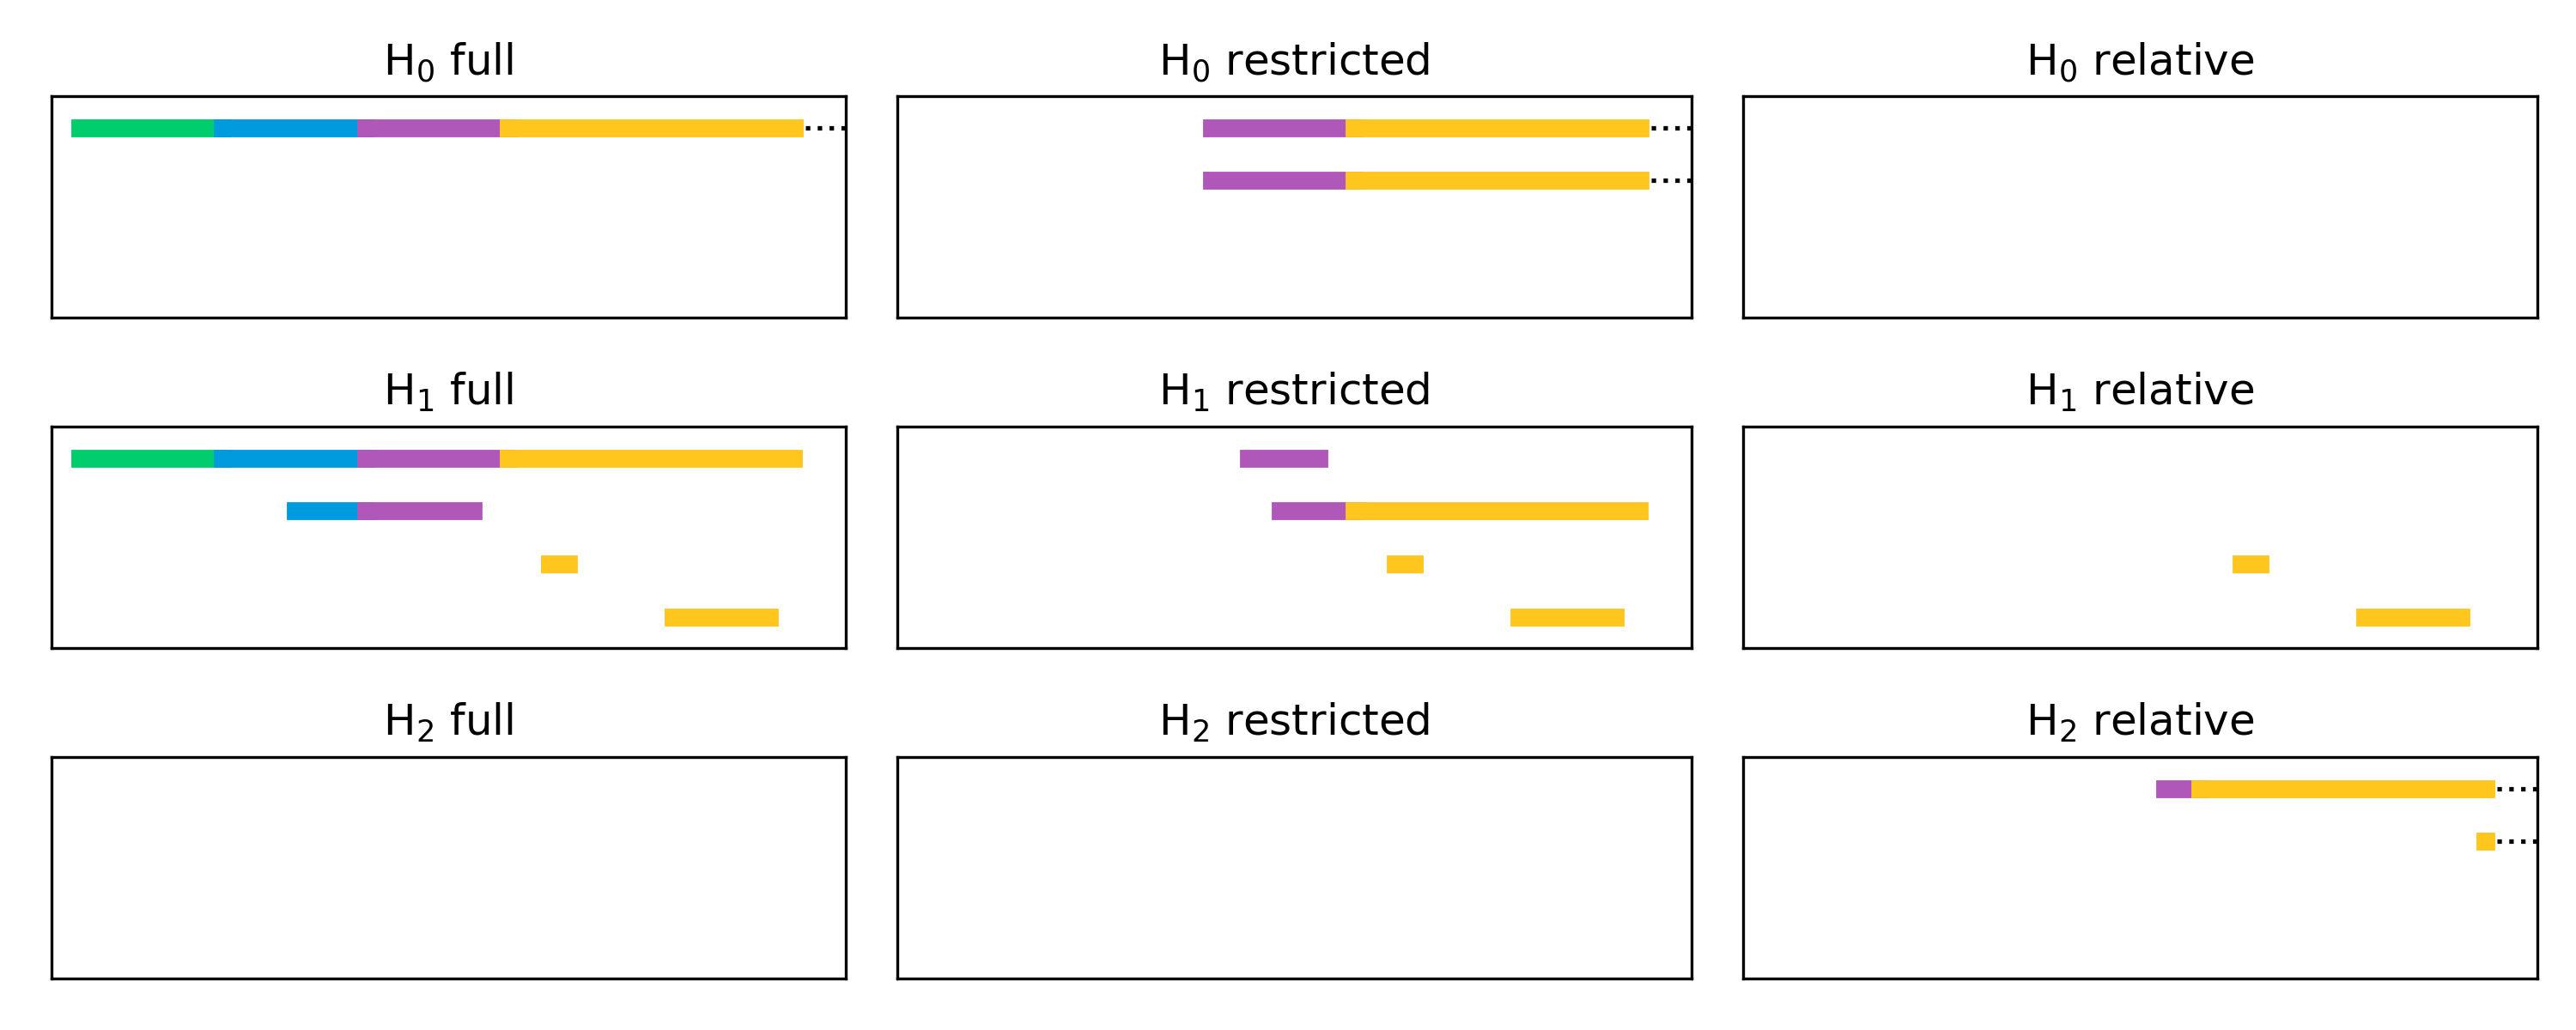
\includegraphics[width=\textwidth]{scripts/figures/barcodes/res_rel.png}
  \end{minipage}
  \caption{Full, restricted, and relative barcodes of the function (left).}% on a $512\times 512$ grid.
    % The restricted barcode is of the function restricted to the region above the blue line.
    % The relative barcode is of the function relative to the blue sub-levelset below the blue line.}
    % We note that the additional features in restricted $\hom_0$ are artifacts of the restriction caused by the approximation.}
\end{figure}

\paragraph*{Outline of Sections~\ref{sec:tcc} and~\ref{sec:middle}}

We will begin with our statement of the TCC in Section~\ref{sec:tcc}.
This requires the introduction of surrounding pairs before proving our reformulation of the TCC (Theorem~\ref{thm:algo_tcc}).
Section~\ref{sec:middle} formally introduces extensions and partial interleavings of image modules which will be used to interleave our approximation with the relative diagram (Theorem~\ref{thm:interleaving_main_2}).

% In Section~\ref{sec:truncations} we address the meaning of the persistent homology relative to a sublevel set and relate it to the sublevel set filtration as a \emph{truncation}.
% Finally, Section~\ref{sec:experiments} investigates the relationships between the relative, truncated, and restricted persistence diagrams through a number of experiments.

% \paragraph{Relative, Truncated, and Restricted Persistence Diagrams}
%
% The goal of Sections~\ref{sec:tcc} and~\ref{sec:middle} is to extend the TCC to approximate the \textbf{relative diagram} associated with a function $f$, defined to be the diagram associated with the filtration $\{(D\subi{\omega}{\alpha}, B_\omega)\}_{\alpha\in\R}$.
% In Section~\ref{sec:truncations} we relate the relative diagram to the \emph{full} diagram of the sublevel set filtration $\{B_\alpha\}_{\alpha\in\R}$.
% Specifically, we define the \textbf{truncated diagram} to be the subdiagram consisting of features born \emph{after} $\omega$ in the full diagram.
% In Section~\ref{sec:experiments} we compare the relative and truncated diagrams to the \textbf{restricted diagram}, defined to be that of $\{D\subi{\omega}{\alpha}\}_{\alpha\in\R}$: the sublevel set filtration of $f\rest_{D\setminus B_\omega}$.

% Specifically, we will select constants $\delta\leq\zeta < \varrho_D/2$ such that, granted the assumptions detailed~\textbf{TODO}, coverage of  can be confirmed by verifying
%
% Theorem~\ref{thm:algo_tcc} uses this condition, along with the established properties of surrounding pairs, to confirm that $Q_{\omega-c\zeta}^\delta$ surrounds $P^\delta$ in $D$ in addition to coverage.
% This allows us to apply excision to \emph{extend} the pair $(P^\delta, Q_{\omega-c\zeta}^\delta)$ to the pair $(D, \E Q_{\omega-c\zeta}^\delta)$ surrounding $D$ in $\X$.
% The resulting inclusion maps facilitate our interleaving of the persistent (relative) homology of $f$ on the pair $(D, B_\omega)$ to that of our sample.
%
% Section~\ref{sec:middle} formally establishes the notion of an extension of a surrounding pair before introducing image modules, and \emph{partial interleavings}.
% These partial interleavings are required due to the static natto relate our approximated boundary \textbf{fuck}%$Q_{\omega-}
%
% At this point we have a set of points $P$ that covers a subset (a \emph{superlevel}-set of $f$) $D\setminus B_\omega$ at scale $\delta$ and a subcover provided by a set of points $Q_{\omega-c\zeta}$ that \emph{surrounds} $P^\delta$ in $D$ at scale $\delta$.
% We can show that the fact that $Q_{\omega-c\zeta}^\delta$ surrounds $P^\delta$ implies that we can apply excision in a way that provides inclusion maps $(D,B_{\omega-c(\delta-\zeta)})\hookrightarrow (D, \E Q_{\omega-c\zeta})\hookrightarrow (D, B_\omega)$ such that the homology of $(D, \E Q_{\omega-c\zeta})$ is isomorphic to that of $(P^\delta, Q_{\omega-c\zeta}^\delta)$\textbf{fuck}
